\section{Generalization}\label{sec_generalization}
In this section we will generaize the described method into a parametric system, i.e. a geometric framework.

\todo{TODO:}
\begin{itemize}
\item introduce section
\end{itemize}

\subsection{Beading strategy}
Depending on the application, the hardware and the materials used we might want to have different strategies for filling a shape with contour parallel toolpaths.
we therefore..


\begin{definition}\label{beading_strategy_definition}
We define a beading strategy as the following set:
$$
\left\{ \alpha_\text{max}, b(d), t(n), t_0(n), W(n, d), L(n, d) \right\}
$$
where
$\alpha_{\text{max}}$ (the limit bisector angle),
$b(d)$ (optimal bead count),
$t(n)$ (transition length)
and
$t_0(n)$ (transition anchor position) have already been defined above.
We introduce here
$W(n, d)$, which gives the sequence of bead widths to cover a distance $d$ using $n$ beads
and
$L(n, d)$, which gives the sequence of toolpath positions as radial distances from the outline to cover a distance $d$ using $n$ beads.
\end{definition}


The following restrictions hold:
\begin{enumerate}
\item $W$ is symmetric: $W(n, d)_i = W(n, d)_{n-i-1}$
\item $L$ is symmetric in $d$: $L(n, d)_i = d - L(n, d)_{n-i-1}$
\item $W_n$ is monotonic and continuous at each bead index $n$ for constant bead count $c$: $0 \leq \frac{\partial W(c, d)_n}{\partial d} < \infty$.
\end{enumerate}


\todo{TODO: Format this in the same way is the list above:}
The transitions lengths should be such that they fit between anchor locations of two consecutive transitions even for a bone with high bisector angle:
$$t_1(n) + t_0(n+1) < \frac{ b^{-1}(n + 1) - b^{-1}(n) }{ \cos \nicefrac12 \alpha_\text{max}}$$
for each $n \in \mathbb{N}$.
See \cref{transition_placement}.

\begin{figure}
\centering
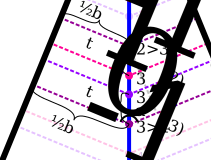
\includegraphics[width=.4\columnwidth]{sources/method/transition_length_limit.pdf}
\caption{
Placement of transition ends (magenta and pink) with respect to the anchor positions of the transitions (purple) on a skeleton segment (blue) with bisector angle $\alpha \approx \SI{135}{\degree}$.
The distance between the anchor position and the upper end ($t_1$) and the distance between the anchor position and the lower end of the transition ($t_0$) should add up to less than the total distance between the anchor positions, which is limited by $\alpha_\text{max}$.
}
\label{transition_placement}
\end{figure}




\begin{definition}
By applying the beading strategy to a skeleton location $v$ and a predetermined bead count $n$ we get a beading $B$, which is defined as the following set:
$$
\left\{ d, n, w_i, l_i  \right\}
$$
where
$d = 2 R(v)$ is the diameter associated with $v$,
$n$ is the bead count,
$w_i$ is the bead width of the bead with index $0 \leq i < n$ counting from the outline inward
and
$l_i$ is the distance of the toolpath location of bead with index $0 \leq i < n$.
\end{definition}




\subsection{Beading strategies}
\todo{This section was moved. Check compatibility with surrounding text.}

Now that we have described a framework for deciding and applying on bead counts and their widths locally, we can introduce several beading strategies which determine the bead count and their widths in different ways.
We can emulate a variety of toolpath generation methods from related literature by meticulously defining new beading strategies.
We also introduce new beading strategies which produce toolpaths with less extremal widths compared to techniques from existing literature.

A beading strategy is defined as a set of some particular variables and functions (\cref{beading_strategy_definition}).
Our beading strategies are based on a preferred width $w_\text{pref} = \SI{0.4}{\milli\meter}$, which is equal to the diameter of the printing nozzle.
Most of the beading strategies we introduce share a common ground:
\begin{align*}
d_\text{max}^\text{transition} &= \SI{1}{\milli\meter} \\
d^\text{discretization} &= \SI{0.2}{\milli\meter} \\
t_\text{beading} &= w_\text{pref} \\
d_\text{max}^\text{intersection} &= \SI{75}{\percent} \\
%
%We use a transition anchor position of
%$$t_-(n) =  t(n) \frac{ b^{-1}(n) - p(n) }{p(n+1) - p(n) }$$
%$$t_-(n) =  t(n) \frac{ b^{-1}(n) - 0.4n }{0.4(n+1) - 0.4n }$$
%$$t_-(n) =  t(n) \frac{ b^{-1}(n) - 0.4n }{0.4}$$
t_0(n) &=  t(n) \left( b^{-1}(n) / w_\text{pref}  - n \right) \\
t(n) &= w_\text{pref} \\
\alpha_\text{max} &= \SI{135}{\degree} \\
L(n,d)_i &= 
\begin{cases}
-\frac12 W(n,d)_i + \sum_{j=0}^i W(n,d)_j & \text{ if } i < \frac12 (n -1) \\
d/2 & \text{ if } i =  \frac12 (n -1) \\
d - W(n,d)_{n-1-i} & \text{ otherwise }\\
\end{cases}
\end{align*}

The transition anchor position $t_0$ ensures that the transitions never overlap with the locations $v$ where $2 R(v) = n w_\text{pref}$ for $n \in \mathbb{N}$.
The transition length $t$ ensures that the center beads don't overlap with the innermost transitioning beads, while keeping the amount of underfill low and keeping the toolpath smooth.
The limit bisector angle $\alpha_\text{max}$ ensures that we don't employ transitioning in shallow wedge regions, which would result in a lot of short odd single bead polylines, which would break up the semi-continuous nature of polygonal extrusion paths.
The toolpath locations $L$ ensure that beads are extruded from the center of where they end up, that the beads don't overlap and that the symmetry restrictions are met.


\paragraph{Naive Beading Strategy}
We can define a beading strategy which emulates the naive method by disabling the marking of edges, so that we never employ transitioning.
\begin{align*}
\alpha_\text{max} &= \SI{180}{\degree} \\
b^-(d) &= 2 \left\lfloor \frac{d}{ 2w_\text{pref}} + \frac12 \right\rfloor \\
W(n,d)_i &= w_\text{pref} \text{ for all } i 
%\\
%L(n,d)_i &= w_\text{pref} \left(i + \frac12 \right) \text{ for all } i < \frac12 n
\end{align*}



\paragraph{Outer bead}
We can emulate the method by \citeauthor{Moesen2011} by carefully choosing how the beading strategy functions deal with the outermost bead.
Also we turn off the reduction of line segments near 3-way intersections, so that the polygonal toolpaths emulate the remaining area to be filled by another path planning technique similar to their technique.

\begin{align*}
d_\text{max}^\text{intersection} &= \SI{0}{\percent} \\
t(n) &= 0 \\
b(d) &=
\begin{cases}
1 & \text{ if } d < w_\text{pref} \\
2 & \text{ otherwise } \\
\end{cases}
 \\
W(n,d)_i &= 
\begin{cases}
d & \text{ if } n = 1 \\
w_\text{pref} & \text{ otherwise } \\
\end{cases}
%\\
%L(n,d)_i &= 
%\begin{cases}
%d / 2 & \text{ if } n = 1 \\
%w_\text{pref} / 2 & \text{ otherwise } \\
%\end{cases}
\end{align*}


\paragraph{Constant bead count}
We can emulate the method by \citeauthor{Ding2016a}, by dividing the feature diameter over the widths of a constant number of beads.
Additionally in order to emulate their definition of branches we mark all segments and in a separate algorithm we unmark the outer bones connected to the outline shape.
Note that this deviation from the proposed framework violates the robustness against small perturbations in the outline polygon, since the topology of the skeletal graph is not stable against those.

\begin{align*}
\alpha_\text{max} &= \SI{0}{\degree} \\
b(d) &= C \\
W(n,d)_i &= d / n \text{ for all } i 
%\\
%L(n,d)_i &= d / n \left(i + \frac12 \right) \text{ for all } i < \frac12 n
\end{align*}



\paragraph{Centered}
We can emulate the method by \citeauthor{Jin2017JMS}, by transcribing how they deviate from the naive tool paths.
We therefore base the beading strategy on the bead count $b^(d)$ defined by the naive beading strategy.
\citeauthor{Jin2017JMS} replace two beads from the naive toolpaths by a single one when the radius between the center and either of those beads falls short of $r_\text{min} = 0.8 w_\text{pref}$.
Conversely, they place an extra bead when the radius between the center and either of the innermost beads exceeds $r_\text{max} = 1.25 w_\text{pref}$.\cite{Jin2017JMS}
We emulate the rounded polygonal path rerouting they define by supplying a transition length which results in a discretized version of the rounded polygon segment.

\begin{align*}
t(n) &= \frac12 w_\text{pref} \\
b^-(d) &= 2 \left\lfloor \frac{d}{ 2w_\text{pref}} + \frac12 \right\rfloor \\
b(d) &= b^-(d) +
\begin{cases}
-1 & \text{ if } b^-(d) w_\text{pref} - d > w_\text{pref} - r_\text{max} \\
1  & \text{ if }  b^-(d) w_\text{pref} - d < w_\text{pref} - r_\text{min} \\
0 & \text{ otherwise}
\end{cases}
\\
W(n,d)_i &= 
\begin{cases}
d - (n-1) w_\text{pref} &\text{ if } i = \frac12 (n-1) \\
w_\text{pref} &\text{ otherwise }
\end{cases}
%\\
%L(n,d)_i &= 
%\begin{cases}
%d / 2 & \text{ if } i = \frac12 (n-1) \\
%w_\text{pref} \left(i + \frac12 \right) & \text{ otherwise }
%\end{cases}
\end{align*}





\paragraph{Evenly distributed}
By taking the advantages of the above two strategies we can define a beading strategy which constitutes a novel toolpathing technique.
We can evenly divide the local feature diameter over the widths of all beads, but choose a local bead count better matching the local feature size.
We determine the local bead count by dividing the diameter by the prefered bead width and rounding to the nearest integer.
This reduces the demands on the system and deviation from mechanical properties caused by beads with extreme deviations from the preferred width.



\begin{align*}
b(d) &= \left\lfloor \frac{d}{ w_\text{pref}} + \frac12 \right\rfloor \\
W(n,d)_i &= d / n \text{ for all } i 
%\\
%L(n,d)_i &= d / n (i + \frac12) \text{ for all } i < \frac12 n
\end{align*}




\paragraph{General distributed strategy}
The evenly distributed strategy can be conceptualized as calculating the total discrepancy $E$ between the actual feature diameter $d$ and the total preferred width $n w_\text{pref}$, dividing the total discrepancy by the number of beads and setting the width of each bead to 
$w_\text{pref} + E / n$.
However, depending on the application we might want a different distribution of widths.
We therefore supply a beading strategy which supports an arbitrary distribution of the discrepancy.
The distribution is determined by some weighing function $M(n.d)$, which defines the portion of the discrepancy to distribute to each bead.


\begin{align*}
b(d) &= \left\lfloor \frac{d}{ w_\text{pref}} + \frac12 \right\rfloor \\
E(n,d) &= d - n w_\text{pref} \\
W(n,d)_i &= w_\text{pref} + E(n,d) \frac{M(n,d)_i}{\sum_{j=0}^{n-1} M(n,d)_j} \text{ for all } i 
%\\
%L(n,d)_i &= d / n (i + \frac12) \text{ for all } i < \frac12 n
\end{align*}


\paragraph{Inward distributed}
For example, we can choose 
$$M(n,d)_i = \max(0, 1 - \frac{1}{N^2} (i - (n-1)/2)^2 )$$
to distribute the discrepancy over the innermost $2N$ beads, and distribute most of it to the inner beads.
See \cref{distributed_comparison}.
That way we limit the region of impact of the distributed strategy to a central region and have the nominal bead width $w_\text{pref}$ in regions farther away.
This limits the impact of transitioning regions so that transitions keep the toolpaths smooth farther away from the central regions. % and it forces most of the beads to have exactly the prefered width.
Moreover, the bead widths equal the nominal bead width for large regions meaning that mechanial properties derived for prints using the naive strategy will still hold approximately.



\begin{figure}
\centering
\setlength{\figwidth}{.45\columnwidth}
\begin{subfigure}{\figwidth}\centering
\includegraphics[width=.8\columnwidth]{sources/validation/wedge_Distributed_pretty_evenly.png}
\caption{Evenly distributed}
\end{subfigure}
\begin{subfigure}{\figwidth}\centering
\includegraphics[width=.8\columnwidth]{sources/validation/wedge_Distributed_pretty_inward.png}
\caption{Inward distributed}
\end{subfigure}
\caption{
Closeup of toolpaths generated with the distributed beading strategies for a large wedge shape.
}
\label{distributed_comparison}
\end{figure}





\paragraph{Widening}
Complementary to any of these strategies we can enforce a minimum feature size at no extra cost in our framework.
Regions where the model is narrower than the nozzle size can be printed with a bead width larger than the model thickness.
We can simply override
\begin{align*}
W'(n,d)_1 &=
\begin{cases}
\max \left( w_\text{nozzle}  ,  W(n,d)_1 \right) & \text{ if } n = 1 \\
W(n,d)_1 & \text{ otherwise}
\end{cases}
\end{align*}




















